\chapter{Analiza emocji i transformacja zbiorów danych}

Dobór odpowiedniego zbioru danych \textit{(ang. dataset)} jest jedną z kluczowych decyzji
podczas pracy z modelami uczenia maszynowego. Dobrze dobrane dane mogą znacząco poprawić jakość
modelu. Z kolei ich nieumiejętne przetwarzanie lub niedopasowanie domeny danych do zadania (np.
trenowanie modelu generującego poezję na tekstach prozatorskich) prowadzi do błędów i
pogorszenia wyników, które często trudno wykryć.

\begin{figure}[h]
    \centering
    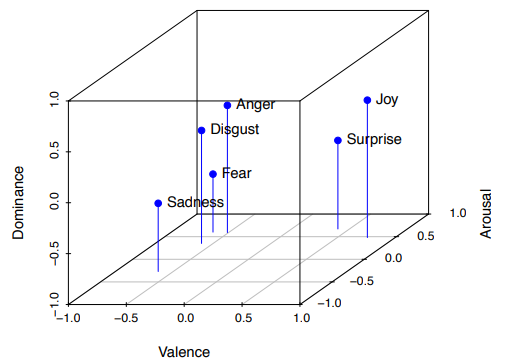
\includegraphics[width=0.7\linewidth]{figures/3/vad.png}
    \caption[Przestrzeń afektywna rozpięta przez trzy wymiary VAD wraz z położeniem sześciu
    podstawowych emocji Ekmana]{Przestrzeń afektywna rozpięta przez trzy wymiary VAD wraz z
    położeniem sześciu podstawowych emocji Ekmana, wyznaczonym przez Russella i Mehrabiana. Źródło:
    \cite{buechel-hahn-2017-emobank}, na podstawie:~\cite{russel_james_evidence}}
    \label{fig:vad_representation}
\end{figure}

\section{Czym jest VAD}
VAD (ang. Valence, Arousal, Dominance) jest wymiarowym modelem emocji, w którym stan emocjonalny
reprezentowany jest przez trzy wartości liczbowe. Wartościowość (ang. \textit{valence}) określa,
jak przyjemna lub nieprzyjemna jest dana emocja, pobudzenie (ang. \textit{arousal}) jak silnie
aktywuje ona organizm, a dominacja (ang. \textit{dominance}) w jakim stopniu osoba odczuwa
kontrolę nad sytuacją. Dzięki temu można odróżnić emocje podobne pod względem walencji i
pobudzenia, np. gniew (wysoka dominacja) od strachu (niska dominacja). W skrócie pozwala opisać
emocje jako punkt w trójwymiarowym ciągłym systemie, gdzie osiami są właśnie te parametry
\cite{vad_description}.

Podejście wymiarowe ma kilka przewag nad modelami dyskretnymi, w których emocji przypisuje się
jedną z ustalonych etykiet. Ze względu na ciągłość skali VAD pozwala opisać nie tylko konkretną
emocję, lecz także jej intensywność oraz stany pośrednie. Dodatkowo wartości liczbowe
umożliwiają wykonywanie podstawowych operacji statystycznych, np. uśrednienie dwóch ocen, co w
przypadku etykiet jest utrudnione lub wymaga dodatkowych założeń. Wadą tego podejścia jest jednak
mniejsza intuicyjność, ponieważ trójka liczb jest trudniejsza do zinterpretowania niż nazwa
emocji.

\section{NRC VAD leksykon}
\label{sec:nrc_vad}
NRC VAD Lexicon v2 jest jednym z największych zasobów opisujących emocje w ujęciu wymiarowym.
Zawiera ponad 55 tysięcy angielskich słów oraz wyrażeń wielowyrazowych, z których każdemu
przypisano trzy wartości (walencję, pobudzenie i dominację) na skali od $-1$ do $1$. Oceny
pochodzą od ankietowanych i zostały zebrane metodą \textit{Best-Worst Scaling}, w której
respondent spośród kilku terminów wybiera ten o największej i najmniejszej wartości danego
wymiaru. Daje to bardziej spójne wyniki niż bezpośrednie ocenianie na skali liczbowej.
Szczegółowy opis procesu zbierania danych i jego rzetelności można znaleźć w
pracy~\cite{mohammad2025nrcvadlexiconv2}.

Leksykon NRC VAD nie sprawdza się jako bezpośredni zbiór treningowy. Zawiera on pojedyncze słowa
i krótkie frazy, więc model trenowany na takich danych nie nauczyłby się uwzględniać kontekstu
zdania. Alternatywą jest użycie leksykonu do zbudowania reprezentacji wejściowej zamiast modelu
osadzeń zdań (ang. \textit{sentence embedding model}), na przykład przez uśrednienie wartości
VAD słów występujących w tekście. Takie podejście, nazywane workiem słów (ang. \textit{bag of
words}), ma jednak tę wadę, że pomija kolejność słów, wieloznaczność i negację. Wyniki
eksperymentów (Tabela~\ref{tab:wyniki_vad}) pokazują, że zamrożony model osadzeń zdań (ang.
\textit{frozen sentence embedder}) osiąga znacznie niższy błąd niż podejście oparte na
leksykonie. % TODO: wstawić liczby i metrykę

\section{EmoBank}
EmoBank~\cite{buechel-hahn-2017-emobank} to zbiór około 10 tysięcy angielskich zdań, z których
każde oceniono w wymiarach VAD na skali od 1 do 5. Oceny wystawiali ankietowani, a autorzy
zbioru zbadali m.in. wpływ perspektywy adnotacji (emocje wyrażane przez autora tekstu a emocje
odczuwane przez czytelnika) na uzyskane wyniki. Szczegóły dotyczące procesu zbierania i
weryfikacji danych opisano w pracy źródłowej.

W porównaniu z leksykonem NRC VAD, EmoBank jest lepiej dopasowany do zadania, ponieważ etykiety
przypisano całym zdaniom, a nie pojedynczym słowom. Ograniczeniem jest jednak skład domenowy
zbioru (Tabela~\ref{tab:emobank_genres}). Fikcja stanowi jedynie około jednej czwartej danych,
a pozostałe zdania pochodzą z tekstów takich jak wiadomości, listy czy przewodniki turystyczne,
co może negatywnie wpłynąć na wynik modelu. Dodatkowo zdania oceniano pojedynczo, bez kontekstu
sąsiednich fragmentów, a w czytaniu książki nastrój zależy właśnie od szerszego fragmentu.

\begin{table}[htbp]
  \centering
  \caption[Rozkład gatunków w zbiorze EmoBank]{Rozkład gatunków tekstu w zbiorze
  EmoBank przed i po filtrowaniu. SE07 oznacza korpus nagłówków prasowych
  z zadania SemEval-2007 (\textit{Affective Text}), a MASC --- zróżnicowany
  gatunkowo podzbiór korpusu OANC (\textit{Manually Annotated Sub-Corpus}).
  Źródło: \cite{buechel-hahn-2017-emobank}.}
  \label{tab:emobank_genres}
  \begin{tabular}{llrr}
    \toprule
    Korpus & Domena & Surowe & Po filtrowaniu \\
    \midrule
    SE07 & nagłówki wiadomości & 1250 & 1192 \\
    \midrule
    \multirow{6}{*}{MASC} & blogi & 1378 & 1336 \\
     & eseje & 1196 & 1135 \\
     & fikcja & 2893 & 2753 \\
     & listy & 1479 & 1413 \\
     & gazety & 1381 & 1314 \\
     & przewodniki turystyczne & 971 & 919 \\
    \midrule
    \multicolumn{2}{l}{\textbf{Suma}} & \textbf{$10\,548$} & \textbf{$10\,062$} \\
    \bottomrule
  \end{tabular}
\end{table}

\FloatBarrier
\section{CR4-NarrEmote}
CR4-NarrEmote to zbiór, który zawiera ponad $200\,000$ adnotacji wykonanych przez ponad $3\,500$ 
osób, przy czym każda adnotacja dotyczy pojedynczego zdania~\cite{piper-budac-2025-cr4}. Największą
zaletą jest pochodzenie tekstów. Popularne
zbiory, takie jak GoEmotions~\cite{GoEmotions} (komentarze z serwisu Reddit) czy
EmoBank~\cite{buechel-hahn-2017-emobank}, opierają się w większości na krótkich formach, a nie
na literaturze narracyjnej. Autorzy CR4-NarrEmote opisują źródło zdań następująco: \textit{„Skupiamy
się na dłuższych formach narracyjnych z dwunastu różnych gatunków literatury pięknej i faktu,
fragmentach obejmujących okres ostatnich 150 lat oraz tekstach pochodzących z różnych obszarów
kulturowych kręgu anglojęzycznego, w tym z Nigerii, Indii i Afryki Południowej, a także z Ameryki
Północnej”} (tłum. własne)~\cite[s.~9774]{piper-budac-2025-cr4}. Ponieważ aplikacja analizuje
fragmenty książek elektronicznych, dopasowanie domeny danych treningowych do
domeny użycia jest tu kluczowe.

Uczestnicy oceniali zdania, wybierając dowolną etykietę emocji (nie byli
ograniczeni zamkniętym zbiorem). Podane etykiety zostały następnie
przekształcone na wartości VAD w skali od $0$ do $1$ z użyciem leksykonu NRC
VAD (sekcja~\ref{sec:nrc_vad}), a potem przeskalowane do przedziału od $-1$
do $1$:
\[
X_{\text{scaled}} = \operatorname{round}(2X - 1,\ 4),
\]
gdzie $X$ oznacza wartość z przedziału $[0, 1]$.
Autorzy udostępniają trzy wersje mapowania etykiet na VAD. Pierwsza (NRC) opiera
się wyłącznie na leksykonie NRC, co zapewnia spójność, ale pomija kontekst:
\textit{„Podejście to, pomimo swojej spójności, posiada braki w reprezentacji
kontekstu (np. wszystkie formy słowa «miłość» są traktowane tak samo)”}
(tłum. własne)~\cite[s.~9775]{piper-budac-2025-cr4}. Druga (NRCBERT) łączy etykietę
nadaną przez uczestnika z kontekstem zdania, wykorzystując Sentence-BERT
(SBERT)~\cite{reimers-gurevych-2019-sbert}. Trzecia (EMO) polega na wytrenowaniu
modelu regresyjnego na reprezentacjach SBERT, bez użycia etykiet uczestników.

Rozkłady wartości uzyskanych poszczególnymi metodami przedstawia
rysunek~\ref{fig:distribution_VAD}. Mapowanie oparte wyłącznie na leksykonie
NRC daje najszerszy rozkład we wszystkich trzech wymiarach, natomiast
wersja trzecia (oznaczona na wykresie jako EMO) jest silnie skupiona wokół
wartości neutralnej, szczególnie dla pobudzenia i dominacji. Wersja druga
(NRCBERT) zajmuje pozycję pośrednią.

\begin{figure}[htbp]
  \centering
  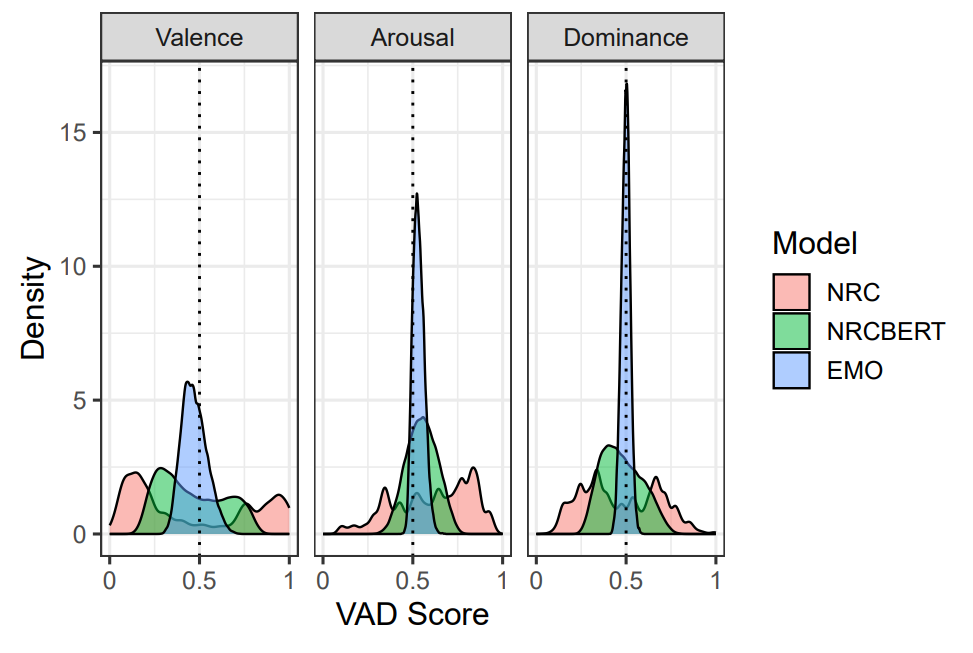
\includegraphics[width=0.8\linewidth]{figures/3/vad_score.png}
  \caption{Rozkłady wartościowości, pobudzenia i dominacji (VAD) dla trzech
  metod mapowania etykiet na wartości VAD. Linia przerywana oznacza wartość
  neutralną~(0,5). Opracowanie na podstawie~\cite[s.~9776]{piper-budac-2025-cr4}.}
  \label{fig:distribution_VAD}
\end{figure}

\FloatBarrier
\subsection{Własna transformacja danych i rekomendacje autorów}
Do trenowania modelu autorzy zalecają użycie wersji drugiej (SBERT oraz etykiety użytkowników) w
przypadku wartościowości (ang. \textit{valence}), oraz pierwszej (mapowania za pomocą leksykonu) 
wersji dla pobudzenia (ang. \textit{arousal}) oraz dominacji (ang. \textit{dominance}):
\textit{„Rekomendujemy użycie NRC dla zadań z pobudzeniem oraz dominacją, jednak dla 
bardziej zbalansowanego przewidywania wartościowości polecamy predykcje NRCBERT”} (tłum.~własne)
~\cite[s.~9776]{piper-budac-2025-cr4}. Podczas badań każdy z badanych mógł opisać dane zdanie
więcej niż jedną emocją, dlatego dla trenowania swojego modelu kilka adnotacji w ramach jednego
zdania przez jednego badanego musiały zostać uśrednione. Według zaleceń autorów do trenowania
modelu zostały użyte BERT\_V, oraz A i D pochodzące z NRC. Finalny zbiór danych użyty do trenowania,
testowania i porównania modeli wyglądał następująco:

\begin{table}[htbp]
  \centering
  \caption{Przykładowe rekordy ze zbioru danych zawierające pierwotne wartości VAD oraz wyznaczone BERT\_V}
  \label{tab:vad_bert_v_sample}
  \begin{tabular}{lrrrrl}
    \toprule
    \textbf{ID tekstu} & \textbf{V} & \textbf{A} & \textbf{D} & \textbf{BERT\_V} & \textbf{Treść tekstu} \\
    \midrule
    100116072 & $-0,6320$ & $0,4980$ & $-0,3627$ & $-0,3724$ & I shouted for her... \\
    \midrule
    100116075 & $-0,6700$ & $0,4700$ & $-0,2220$ & $-0,2144$ & I wish we could... \\
    \midrule
    ...\\
    \bottomrule
  \end{tabular}
\end{table}
Kolumna V pozostała dla późniejszych testów i porównania modeli między sobą. Po transformacjach
zbiór posiada $38\,209$ wierszy zredukowanych z ponad $200\,000$ adnotacji, poprzez agregacje ocen użytkowników w kontekście jednego zdania oraz odrzuceniu rekordów bez etykiet, co po losowym
podzieleniu zbioru na standardowe podzbiory daje:
\begin{table}[htbp]
  \centering
  \caption{Podział zbioru danych}
  \label{tab:train_dev_test}
  \begin{tabular}{lrrr}
    \toprule
    & \textbf{Podział} & \textbf{Liczba danych [wiersze]} & \textbf{Opis} \\
    \midrule
    train & 70\% & $26\,747$ & Zbiór użyty do trenowania modelu\\
    \midrule
    dev & 15\% & $5\,731$ & Zbiór używany do porównania wyników modeli\\
    \midrule
    test & 15\% & $5\,731$ & Zbiór do testowania modelu\\
    \bottomrule
  \end{tabular}
\end{table}

\section{Podsumowanie i ograniczenia}
Do dalszych prac wybrano zbiór CR4-NarrEmote. Jego zaletą jest pochodzenie
tekstów, czyli literatura narracyjna, bliska domenie aplikacji, oraz większy
rozmiar po przygotowaniu danych (tabela~\ref{tab:datasets_comparison}).
Zbiór GoEmotions pominięto, ponieważ jego etykiety to dyskretne kategorie
emocji, a nie wymiary VAD, co wymagałoby dodatkowej konwersji.
\begin{table}[htbp]
  \centering
  \caption{Porównanie rozważanych zbiorów danych}
  \label{tab:datasets_comparison}
  \begin{tabular}{lllll}
    \toprule
    \textbf{Zbiór} & \textbf{Ostateczny rozmiar} & \textbf{Domena} & \textbf{Etykiety} & \textbf{Język} \\
    \midrule
    CR4-NarrEmote & $38\,209$ wierszy & literatura narracyjna & VAD & angielski \\
    EmoBank       & $10\,063$ wierszy & wiele gatunków        & VAD & angielski \\
    \bottomrule
  \end{tabular}
\end{table}

\FloatBarrier
Wybrany zbiór ma jednak istotne ograniczenia. Największym z nich jest
jednojęzyczność: oba rozważane zbiory są anglojęzyczne, więc zastosowanie
modelu do polskich e-booków wymaga tłumaczenia tekstu lub modelu
wielojęzycznego Po drugie, zbiór zawiera oceny pojedynczych zdań, a aplikacja analizuje ciągły
tekst, więc wpływ kontekstu nie jest bezpośrednio mierzony. Wreszcie, oceny
emocji są subiektywne i mogą zależeć od kultury annotatorów.

